
\documentclass[a4paper,12pt,bibtotocnumbered, twosite]{scrreprt}

\usepackage[utf8]{inputenc}
\usepackage[T1]{fontenc}
\usepackage{amsmath}
\usepackage{graphicx}
\usepackage{placeins}
\usepackage{float}
\usepackage{array}
\usepackage{booktabs}
\usepackage{wrapfig}
\usepackage{cite}
\usepackage{etoolbox}
\usepackage{enumitem}
\usepackage{siunitx} 
\usepackage[hyphens]{url}
\usepackage[english]{babel}
\usepackage{acronym}
\usepackage{braket}
\usepackage{sidecap}
\usepackage{booktabs,array}
\newcolumntype{N}{>{\bfseries\footnotesize}l}
\usepackage[table,xcdraw]{xcolor}
\usepackage{subfigure}
\usepackage{subcaption}
\usepackage{grffile}
\usepackage{xcolor}
\usepackage{framed, color}
\usepackage{empheq}
\usepackage{fancyhdr}
\usepackage{amssymb}
\usepackage{floatflt}
\usepackage{tikz}
\newcommand{\circled}[2][]{
            \tikz[baseline=(char.base)]{
            \node[shape=circle,draw,inner sep=0.2pt] 
            (char) {\phantom{\ifblank{#1}{#2}{#1}}};
           \node at (char.center) {\makebox[0pt][c]{#2}};}}
\robustify{\circled}
            

\setcounter{tocdepth}{4} 
\setcounter{secnumdepth}{4} 
\usepackage{geometry}
\geometry{a4paper,left=30mm,right=30mm, top=3cm, bottom=3cm} 

% Spezialpakete
\usepackage{epigraph}
\setlength{\epigraphrule}{0pt} % kein Trennstrich


\usepackage[onehalfspacing]{setspace}
\usepackage[pdfborderstyle={/S/U/W 1}]{hyperref}

% Seitenmarkierungen 
%\newcommand{\phv}{\fontfamily{phv}\fontseries{m}\fontsize{9}{11}\selectfont}
%\usepackage{fancyhdr} % Schickere Header und Footer
%\pagestyle{fancy}

%\fancyhead[L]{\phv \leftmark}
%\fancyhead[L]{\phv \nouppercase{\leftmark}}
%\fancyhead[R]{\phv \thepage}
% Unten besser auf alles Verzichten
%\fancyfoot[L]{\textsf{\small \kurztitel}}


\newcommand{\titel}{Single Shot correlation in VMI- TOF measurements on He  nanodroplets at MIR femtosecond laser pulses}
\newcommand{\welchethesis}{To Applied for the Grade of Master of Science in Applied Physics}
\newcommand{\thesisofwas}{Thesis}
\newcommand{\welchesInstitute}{Faculty of Physics}
\newcommand{\welcheUni}{Albert-Ludwigs-Universität Freiburg}



\newcommand{\kurztitel}{Template Abschlussarbeit}
\newcommand{\autor}{Cristian Enrique Medina Hernandez}
\newcommand{\datee}{15. febrary 2019} % Abgabedatum
\newcommand{\place}{Freiburg}
\newcommand{\referent}{ Prof.\ Dr.\ Marcel\ Mudrich and Prof.\ Dr.\ Frank\ Stinkermeier  } 



%------------------------------------

\begin{document}


\begin{titlepage}
\centering

\includegraphics[width=7 cm]{logo}

\begin{center}    
    {\LARGE .} \\[0.5cm]
    {\large .} \\[5mm]
    {\large  \thesisofwas\ \welchethesis} \\ \welcheUni \\ \welchesInstitute  \\[5mm]
    \rule{\textwidth}{2pt}\\[0.5cm] 
    {\begin{spacing}{1.15} \huge \bfseries \titel \\
    \end{spacing}}
    \rule{\textwidth}{2pt}    
    \vfill 
 
     



    \begin{tabular}{ll} 
      Presented by & \autor \\
      Date & \datee \\
      Referent & \referent \\
    \end{tabular}  

\end{center}
    
\end{titlepage}
%---------------------------------------------------------------------


\chapter*{Abstract}

In this thesis a new data acquisition method is explained  for correlate single shot VMI-TOF measurements on He droplets ionized by a MIR femtosecond laser.  Until now VMI images and TOF data are always treated in a statistical way. Whit these new method we expect to have some better correlation for single explosion and relate each of the event from a  individual way, having specific information that could be lost in the statistical method.
The correlated data is acquired by triggering the VMI camera and the TOF oscilloscope with the laser trigger, so both acquisitions begging and end after the same laser pulse. Results for the energies..............here a resumy of the results..........

\newpage

\tableofcontents
%%%%%%%%%%%%%%%%%%%%%%%%%%%%%%%%%%%%%%%%%%%%%%%
\chapter*{List of abbreviations}
\begin{acronym}[DARAM]

 \acro{ATI}{above threshold ionization}
 \acro{BSI}{barrier suppression ionization}
 \acro{CCD}{Charge-coupled Device}
 \acro{CPA}{Chirp Pulse Amplification}
 \acro{CWL}{Central wavelength}
 \acro{EM}{Electro Mechanics}
 \acro{LASER}{Light Amplification by Stimulated Emission of Radiation}
 \acro{LT}{Langmuir-Taylor}
 \acro{MCP}{Micro Channel Plate}
 \acro{NIR}{Near Infrared}
 \acro{pBASEX}{polar Basis Set Expansion}
 \acro{PID}{Proportional – Integral – Derivative}
 \acro{TBR}{Three Body Recombination}
 \acro{TOF}{Time of flight}
 \acro{VMI}{Velocity Map Imaging}
 \acro{VUV}{vacuum ultra violet}
 \acro{XUV}{Extreme ultraviolet}
  
\end{acronym}
%%%%%%%%%%%%%%%%%%%%%%%%%%%%%%%%%%%%%%%%%%%%%%%
\cleardoublepage\pdfbookmark{\contentsname}{toc}

%%%%%%%%%%%%%%%%%%%%%%%%%%%%%%%%%%%%%%%%%%%%%%%


\section{Introduction}

Physicists have always wonder to explain and resolve dynamic processes in short scale times, so initial conditions of processes can be  describe in a time  evolution scale. Describe any system like this requires to acquire data in shorter windows of time, for example a film is only a consecutive sequence of  photographs that recreate a large time laps in a smaller time scale pics. For  atomic physics, we are talking about a micro-cosmos that varies from microseconds, i.e several bodies dynamics, to  attoseconds  for atoms,where time scales can go down to $10^{-9}$ $s$, requiring to create measurement methods capable to record in shorter time, while the experiment have to be done in a controllable way to ensures its reproductivility, as any scientific method.

The time window of dynamics of a sytem is related to  quantum dynamics, in a simple view also to its size. For dynamics happening in a molecule or a many body system interaction, the time window can oscillate between  microseconds to fentoseconds, although for millielectronvolt-scale $(meV)$ energy spacing of vibrational energy levels implies that molecular vibrations occur on a time scale of tens to hundreds of femtoseconds. The motion of individual electrons in semiconductor nanostructures, molecular orbitals, and the inner shells of atoms occurs on progressively shorter intervals of time ranging from tens of femtoseconds to less than an attosecond. Motion within nuclei is predicted to unfold even faster, typically on a zeptosecond time scale.

To achive this higth resolution in space and  time physicist have challenged to create systems with a well controlled spatial and temporal gradient. Fortunately nowadays, laser pulses can research up to extreme non-linear optical processes, produccing single aisolated  pulses of ultra violet(UV) waves as short as 67 $as$ \cite{zhao_tailoring_2012}.  Such fast pulses open up the possibility of time resolved measurements fort short processes like electron dynamics.  However, to do this, experimental schemes must be devised that allow these new light sources to be used to perform measurements on the microcosmos. In particular, in the last few years,  many studies at atom- and molecule-clusters had been published, From mid-infre red (NIR) interaction to UV or XUV pulses, that not just lead to a broad spectra to study but also to a large range of possible applications such as the generation of  energetic electrons and ions in the keV-regime \cite{fennel_laser-driven_2010}, as well as intensive XUV and attosecond pulses \cite{stebbings_generation_2011}. Laser pulses with peak intensitiesof up to $10^{21}$ $W/cm^{2}$  are available nowadays \cite{mikaberidze_atomic_1981} commercially so the difficulty and expensive of the experiments source also are easy.

But this is never enough, Lasers is just one huge step in order to control and ignite atomic processes in controlled standard. Other step needed is how to acquire the information we want. For this purpose several techniques are available  depending the nature of the process. For this particular  work we are interested in two  techniques, Velocity map image (VMI) and Time of flight (TOF).
Since its invention, this techniques  has become two of the most commune and important measurement techniques in high energies physics.
%%Mising more info of VMI and TOF)
But detecting a signal is just one part of the job, the new laser advances like the  generation of coherent high-intensity laser pulses with intensities up to $10^{22} W/cm^{2}$  allow multiphoton ionization that allows to get time resolved measurements. These advances have enabled the development of new research areas, as well as the investigation of ultrafast dynamics in highly excited matter to nanometer size.

In this thesis we focus our efforts  on the ionization process by Mid Infrared (MIR) femtosecond pulses in doped $He$ clusters. The interaction of the dopant with the Laser field result in a energy transfer to the droplet that ignite a ionization process, known as a nanoplasma. This resonant interaction of the laser field with a collective oscillation of the electrons in the plasma is driven by the laser field \cite{fennel_laser-driven_2010}. This process, caused predominantly by electron impact ionization, makes an avalanche-like ionization of the atoms in the cluster, leading to a heating of the plasma and, as a result, to hydrodynamic expansion and Coulomb explosion. To the analysis of this process we studied the electrons as well as the ion's resulting in the coulomb explosion. A velocity map imaging and a Time of flight technique are set up in parallel to acquire the data and reconstruct the initial energies and configuration of the plasma in study. 
In the First chapter we will present a brief introduction to the Droplet He generation, a short plasma interactions as a basic background of coulomb ionization in order to understand the physical meaning.
In the second chapter a more detailed explanation of the set-up used is done. Showing from the creation of the He droplets process to its detection , going thorough the doping, and ignition process.
For the third chapter a detailed explanation on the correlation method for the VMI-TOF measurements is done, and showing the set-up of the data acquisition and its advantages.
In the fourth chapter we present the correlated data and its analysis. Finally the last chapter we present the conclusion of the experiment itself also as the data analysis and future works will needed to improve this process as well.


\newpage  
% !TeX spellcheck = en_GB
% !TeX spellcheck = en_US 
\chapter{Theoretical Background}

In this chapter we will present all the theoretical background necessary for the development of this project, from the theory and creation of the He droplets to the physics behind the plasma and coulomb explosion process to the detection techniques. In order to guide the reader in an organised way, the chapters are organized in a way that follow the processes necessaries to the performance of the experiment. this means that all the chapters explained in here occurrence in the same order during the experiment.


\section{Helium Nanodroplets}

The combination of cryogenic matrix isolation, discovered in 1954 \cite{whittle_matrix_1954}, and the now well defined properties of Helium ($He$), specially its superfluidity face discovered in 1937 by \textit{Kapitza et. all}            \cite{kapitza_viscosity_1938}, have as consequence one of the most powerful and flexible tool in physics, the helium nanodroplets.
Helium nanodrops  have unique properties that makes it  very suitable for the cluster and nanophysics experiments in the last decades. For example, they do not exhibit any optical transitions in the entire infrared, visible and ultraviolet range. They can readily pick up atoms and molecules and  form complexes from the species embedded in their interiors, or on their surfaces and act as a ideal matrix for atom, molecules and clusters isolation. \cite{stienkemeier_spectroscopy_2006}\cite{toennies_superfluid_2004}.
The size of a He cluster can go from of a few thousands up to $10^{8}$ of atoms, and reach temperatures at   ultra cold temperature regime (close to 0.37$K$ \cite{toennies_spectroscopy_1998})\cite{enss_low-temperature_2005}.
Two main advantages of this  cooling properties arise. First,  dopants in the He nanodroplet are set to their absolute vibronic ground states, avoiding all other possible espectra and stablishing the cluster in a specific state, more important, the fast cooling helps to the formation of isomers that are difficult or impossible to generate with other methods \cite{nauta_nonequilibrium_1999}. Second, because the superfluid fase of the He nanodroplets\cite{grebenev_superfluidity_1998}, the bond between dopants and He is weak. Therefore, in contrast to spectroscopy in other matrices with higher temperatures, the optical transitions of many dopants are barely influenced by the He matrix \cite{toennies_superfluid_2004}. 
The theory of  He superfluidity will not be part of this section, this imformation is well documented in other sources, and here we are based on ref.\cite{enss_low-temperature_2005} where all theory is well presented to the reader. In the next section we will dedicate a bigger effort on explain the theoretical and technical background of the He nanodroplets creation as well as the physical and technical process to doped it. 

\subsection{He Nano droplets production}

At room temperature, helium is a light inert gas. It is odorless, colorless, tasteless, and after hydrogen, the second most abundant element in the universe.  \cite{enss_low-temperature_2005}. It have a simple 2 atoms structure, exhibing numerous exotic phenomena whose theoretical descriptions are rather complex in many cases, i.e it characteristics of  a quantum fluid. From helium exist  two stable isotopes $^{3}He$ and $^{4}He$.  $^{4}He$ has two electrons, two protons and two neutrons, no nuclear spin and no total spin, pertaining to the bosonic family, while $^{3}He$ with only one neutron has a spin of $I = 1/2$ and belongs to the fermions \cite{atkins_liquid_2014}.

The bosonic state $_{4}He$ is specially of interest, at  temperature T$\leqslant$2.8K and under normal pressure has a phase transition from "normal liquid" He-I to super liquid He-II \cite{swenson_liquid-solid_1950}, in which the helium can be described by a Bose-Einstein condensation. Even the fermionic $^{3}He$ exhibits this phase transition at T$\leqslant 0.03K$ \cite{halperin_properties_1978}.

The superfluidity of $He-II$, at temperatures close to absolute zero, brings with it some unique features. The essential Properties for this include an almost disappearing viscosity in the superfluid phase, weak interaction, very efficient cooling, and the Transparency for electromagnetic radiation up to wavelengths in vacuum ultraviolets (VUV) Spectral range \cite{enss_low-temperature_2005}. Helium has therefore in the complete visible spectrum no transitions from the ground state. Through the noble gas configuration, helium has a spherically symmetrical electron distribution \cite{lewis_helium_2014}, it can hardly be polarized and is the least reactive of all the elements.

\subsubsection{Helium Droplets}

The production He droplets had to overcome first one principal problem, its liquefaction. At the end  of 19th century many gases were liquefied for the first time by applying pressure at room temperature. However, for He and hydrogen, this method was not successful. In 1922 Kamerlingh Onnes reached temperatures below $1K$ by reducing the vapor pressure above liquid helium to about $2*10^{-5}$ bar with a series of pumps \cite{van_delft_discovery_2010}. The Joule–Thomson effect \cite{weinberger_discovery_2013} is in this case the responsible for Onnes experiment to reach this low temperatures. The basic idea is that under suitable conditions a gas in expanding performs work against its internal forces. Basically the gas is expanded through a small nozzle thermally isolated from its surroundings. The expansion under theses conditions takes place at constant enthalpy, since the expansion nozzle performs no work. following the next relation:

\begin{equation}
W= H_{1}-H_{2} = (U_{1}+p_{1}V_{1})-(U_{2}+p_{2}V_{2})
\end{equation}

where H is the entalpy before and after, $U=\dfrac{3}{2}Nk_{b}T$ for ideal gases and $pV=Nk_{b}T$ \cite{enss_low-temperature_2005}. Under Joule–Thomson effect conditions, $W=0$ so $H_{1}=H_{2}$, this expansion leads to a cooling or a warming and under certain conditions, becomes supersaturated. As a result, condensation takes place and a beam of clusters is formed.

Helium nanodroplets are typically produced by a continuous or pulsed adiabatic Expansion of pre$-$cooled helium through a small aperture from a reservoir into a vacuum  \cite{stienkemeier_spectroscopy_2006}. In this process a droplet jet is formed, and its characteristics (blasting speeds and size distribution) can be changes due the manipulation of the set$-$up. For example, $\bigtriangleup$ pressure between the reservoir and the vacuum chamber (usually in the range of a few to $10MPa$) , the nozzle temperatures(from a few K to $T \leqslant 40K$) or the nozzle size (with pinholes of diameter rounding  $5-20 \mu m$).


\begin{figure}[h!]
\centering
	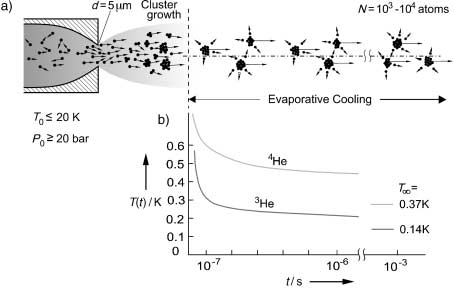
\includegraphics[width=0.6\textwidth]{../Images/jet_scketch.png}
	\caption[Scheme for a nozzle expansion]{ a) Schematic representation of the processes leading to the formation and subsequent cooling of helium droplets in a gas expansion. b) Calculated dependence of the droplet temperature on time for $^{4}He$ and $^{3}He$ droplets after they have left the cluster, taken from \cite{toennies_superfluid_2004}	}
	\label{img:jet}	
\end{figure}

\begin{figure}[h!]
\centering
	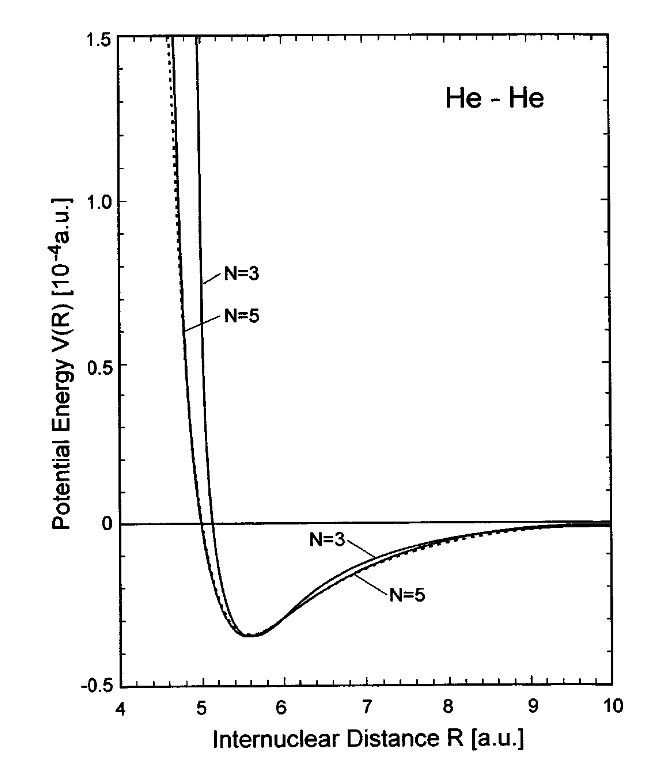
\includegraphics[width=0.5\textwidth]{../Images/waanderwaal_hehe.PNG}
	\caption[Waan der Wall He-He potential]{ Waan der Wals potential for He-He interaction}
	\label{img:WanderHe}
\end{figure}


When the Helium expands from the nozzel, its thermal energy is transform in kinetic energy of a supersonic flow field. After the expantion into the vacuum, the gas becomes supersaturated and condensations starts to occurs, creating the beam clusters. This clusters are made of atoms or moleulces held togueter by Wannder wals fores, in this case He-He interaction, that share the same kinetic vector. This means that the two particules travel as close and parallel to each other that a bonding is possible, see fig \ref{img:WanderHe}. From the reference frame of the cluster, each of its molecules are close to cero movments, in He this enhace the conditions to be liquid and in consecience superfluidity is achive  \cite{hagena_cluster_1972}.
 

There is no mathematical approach of the physics behind this cooling expansion but usually, Raleigh scattering measurements in combination with an empirical scaling law \cite{hagena_cluster_1972} are used to estimate the mean cluster size giving a certain degree of control over the cluster size distribution by adjusting the nozzle width and the source pressure. The droplet size distribution during supersonic expansion in the follows a log-normal distribution of the form \cite{harms_density_1998}.

\begin{equation}
p(N) = \frac{1}{\sqrt{2\pi}N \sigma} \exp  \left[- \frac{(ln(N/N_{0})^2}{2\sigma^2} \right]
\end{equation}
Where \textit{N} is the number of atom in the cluster, $\sigma$ is the distribution width and \textit{$N_{0}$} is the most likely numbers of atoms. Following it give a mean value.
\begin{align}
\bar N = \exp  \left(\mu+\frac{\sigma^2}{2} \right)
\end{align}
With a half width maxima of \cite{harms_density_1998}
\begin{align}
\sigma N_{\frac{1}{2}} = \exp \left( \mu - \sigma ^2 + \sigma \sqrt{2 ln(2)} \right) - \exp \left(  \mu - \sigma ^2 - \sigma \sqrt{2 ln(2)}  \right)
\end{align}

\begin{figure}[hbtp] \label{fig:ExpRegim}
\centering
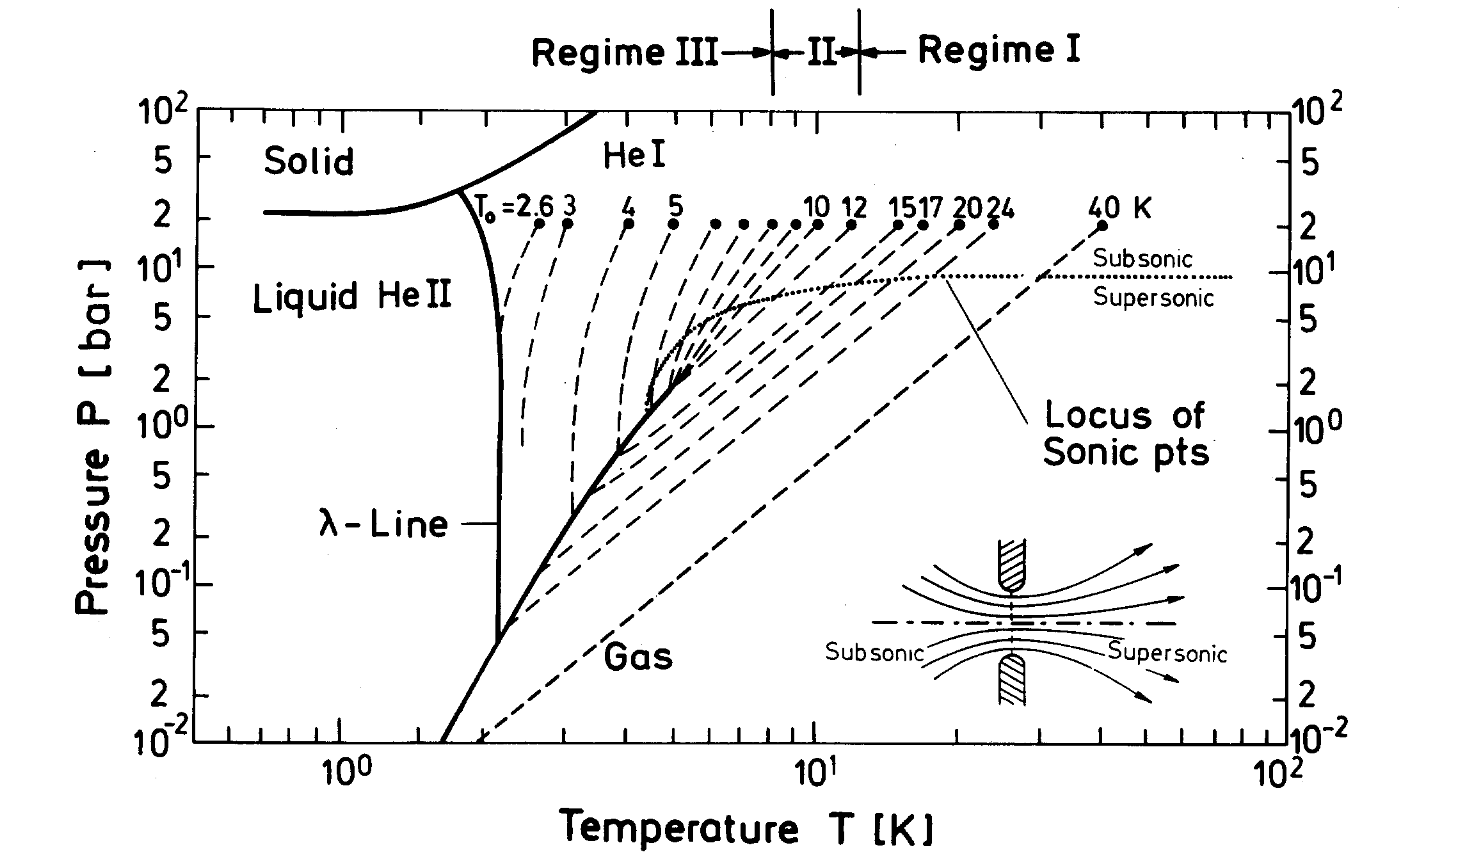
\includegraphics[width= 13 cm]{../Images/expansion_regimes.PNG}
\caption[Phase diagram for Expantion regimens]{Expansion regimes. Pressure-Temperatur phase diagram for $^{4}He$ for Nozzle beam expansions starting from a stagnation of 20 bar and a temperatures. As dicusse, quialitatively different behaivors are shown for the regime I - II and II where  starting in the gas phase,  near the phase trnasition respectivelly. taken from \cite{buchenau_mass_1990}. }
\end{figure}

As show in Figure \ref{fig:ExpRegim} The conditions in the He (pressure, temperature and nozzle size) in the free expansion will determine the characteristics of our final He beam. From Here three main regimes can be define.

Regime I or sub-critical expansion, begins in the gas phase and leads to droplet formation via condensation. this is the case of most expansions since the pressure are located below the critical pressure $P_{c}$.
Regime II, also called as critical expansion, is basically  and interminable regime that includes all trajectories which are near the critical point, leading to random expansion and difficult control of the beam due the large fluctuations in density.
Regime III, the  supercritical expansion, starts at low temperatures where the He stops behaving as an ideal gas, expecting flashing or cavitation  breaking up the liquid drops jet. \cite{buchenau_mass_1990}

super-critical and sub-critical regimes have been studies  in the last several years and  are clearly identified in the resulting size distributions. Figure \ref{img:dropletSize} shows that supercritical expansion forms large droplets (usually between $20-100 nm$ diameter) while a sub-critical expansion is suited to generate small droplets (around $5-10 nm$).  A simple relation that can be done to calculate the size or number of atom in a Custer is using. 

\begin{equation}
r=N_{1/3} * \rho A
\end{equation}

Where $r$ is the radius of the beam, $\rho$ is the density, in thhis case of He $\rho =0.0022 A $ \cite{stringari_systematics_1987}, but this approximation is not exact due the variation Of He density at this temperatures. As expected in both regimens for creating larger helium nano droplets, higher helium pressure and lower nozzle temperature are used. For our experiment a $5 \mu m$ nozzle was used at temperature oscillating between $11-15 K$, at pressure of $30 to 50$ bar.

\begin{figure}[hbtp]
\centering
\label{img:dropletSize}
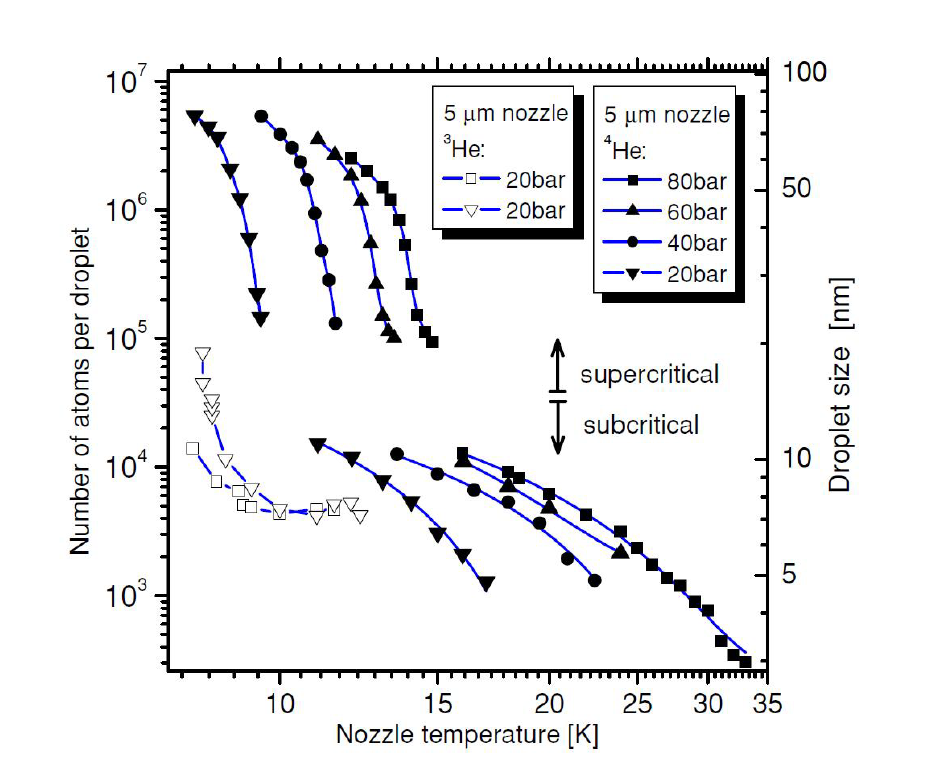
\includegraphics[scale=0.4]{../Images/sizes_regimen.PNG}
\caption[Expantion droplets Regimens]{Sizes of the $^{4}He$ droplets  as a function of nozzle temperature T and  pressures, based on \cite{toennies_spectroscopy_1998}, using a $5 \mu m$ nozzle. The su and super critical regimes are clearly diferenciated. Taken from \cite{stienkemeier_spsectroscopy_2006}}
\end{figure}


\subsubsection{Composite Clusters}

We can define a composite cluster or doped cluster, as a atom  bulk of one material that contains one or more different atomic elements. Usually in homogeneous clusters the main interest is their properties behaviour as a function of its size, but for doped clusters, the interaction between the elements creates new degrees of freedom that makes more complex its behaviour. For example, the new composite will have different structural properties due the spatial distribution of the species. Hence, composite clusters exhibit a more diverse behaviour and offer more opportunities to study different characteristics the material.

The first problem to overcome in composite cluster  is how to create them. Two techniques can be used. The first one, is the co expansion of
a previously mixed gas \cite{tchaplyguine_variable_2004} or the He cluster is produced first and then crossed with an atomic beam of the doping species.

The first technique  involves several technical problems, depends on possible interactions between the elements, the condensation ranges of the bulks and even in the  affinity  of the materials. One of the most used techniques, and the one used in this study is the one called pick-up technique \cite{gough_infrared_1985}. The idea is simple, as well as a snowball on its way downhill collects or pick-up more snow. The He cluster, after being directional selected through a Skimmer,  passes through a doping cell with a dopant gas at low densities ($10−2 Pa$) \cite{stienkemeier_spectroscopy_2006}. As a result, the gas atoms that are along the droplet cross sections will be captured by the beam and travel with it. The probability for helium droplets to collect $k$ atoms or molecules via inelastic collisions depends on the length of the oven cell $l$, the cross section of the droplets $\sigma$, and the particle density inside the cell $n$. As $l$ and $\sigma$ remains constant, varying the density in the doping cell can  regulated the abundance of $k$, following the Poissonian statistics:

\begin{equation}
P_{k}(l,n,\sigma)=\dfrac{(ln\sigma)^{k}}{k!} e^{(-ln\sigma)}
\end{equation}

Two important properties of these relation can be infer. First the maxima of different cluster sizes  are equidistant, $n_{max}=\dfrac{k}{l\sigma}$ and second, the exponential function in equation  becomes  nearly  one for  small  particle  densities \cite{bunermann_modeling_2011}.

Every pick-up process leads to an energy transfer to the droplets. As the dopant rapidly cool down to their, it means a transfer of energy to the He causing an  evaporaton of  helium atoms to keep the temperature unchanged. This He evaporation or "shrinkage", leads to a decrease of the cross section of the droplet and the probability to collect a further particle is  reduced. The involved energy is composed of the following contributions \cite{bunermann_modeling_2011}.

\begin{equation}
E=\langle E_{kin}\rangle + E_{in} + E_{binding} + E_{cluster}
\end{equation}

where

\begin{equation}
\langle E_{kin}\rangle \approx \dfrac{3}{2}k_{b}T + \dfrac{1}{2} m v^{2}
\end{equation}

is the kinetic energy of the droplet depending on it mass and velocity and temperature in the gas cell.

At a certain energy entry, the complete droplet evaporates if to may dopping acces to it. With $E_{kin}$ the average kinetic energy, $E_{in}$ the internal. Several studies have studied the $E_{binding}$ with $^{4}He$, given a broth number of materials to work with.. it also importat to take into acount that the binding energy include the cluste dopant binding as well as the dopant-dopant relation.\cite{toennies_spectroscopy_1998}. Acommung energy bounding for example $Xe-He$ is arround $26.9 meV$\cite{lewerenz_successive_1995}, or $He-H_{2}O$ is about $0.1 eV$ \cite{lewis_helium_2014}, AA more detailed table of all the energy bounding energy used in this study can be found in the appendix.

  
\section{Cluster-Intense Fields  Interaction}

To understanding of the interaction atoms-fields have been study broadly in physics since Einstein Photoionizasion Theory \cite{einstein_uber_1905}, that gives a base on all the quantum electrodynamics theory. The basics unders this theory is the behaivour of ligth as a electromagnetic field where the electron as a bounded charge in the atom can be afected.  This quantum dynamic theory is well understood since 1957 for small atoms, with one, two or few electrons \cite{a._bethe_quantum_1957}, but still big molecules and atoms have been challenging scientific for years. In this chapter we will give a brief introduction to the photoionization process, explaining at the same time multi-photoionization and tunnelling precesses, so we can finish with a more detailed presentation of Strong field interaction with clusters and the Keldish theory.


\subsection{PhotoIonization for single atoms}

The process of photoionization describes the leaving of an electron from its bound state  into the continuum by interaction with electromagnetic field radiation\cite{berkowitz_photoabsorption_1979}. The atomic bounded electrons while going through an electro magnetic field, in our case the laser beam,  can absorb enough  energy to get excited and fly away from the nucleus. A bound electron only can escape from an atom by absorbing photons its energy exceeds the binding energy of an electron \cite{einstein_uber_1905}. When the photon energy of the laser is smaller than the ionization potential of the target, the electron can absorb two or more photos in the ionization process, this is called Multi photon ionization (MPI). Another possible process is called, tunnelling ionization, where due the quantum mechanic properties of the electrons under certain conditions absorb enough energy enough to be on an above threshold regime and due it quantum dynamic properties it can escape from it bounds via tunnelling.

There is a variety of theoretical approaches to describe interaction of  laser fields with atoms. The Hamiltonian of the system of $N$ particles (ions and electrons) with pair-wise Coulomb interactions under the action of an external time-dependent electric field has the form:
\begin{equation}  \label{eq:hamiltonian}
\centering
H = \displaystyle\sum_{1 \leqslant i \leqslant N}^{} \dfrac{P_{i}}{2m_{i}} + \displaystyle\sum_{1 \leqslant i < j \leqslant N}^{} \dfrac{q_{i}q_{j}}{\mid r_{i}-r_{j} \mid} + \displaystyle\sum_{1 \leqslant i \leqslant N}^{n} q_{i}r_{i}\varepsilon(t)
\end{equation}

where $ r_{i,  p_{i}} $ and $ q_{i} $ are the coordinates, momenta and charge of the particles including the interaction between the classical electric field and $ \varepsilon(t) $ where \cite{mikaberidze_atomic_1981}

\begin{equation}
\varepsilon(t) = \varepsilon_{0} e_{z}cos(\omega t + \varphi)
\end{equation}

The proces that drives ionization can be divide on two regimes, a quantum electrical regime and a clasical one. \cite{karnakov_strong_2009}. Equation \ref{eq:hamiltonian}, use the non-relativistic approximation and neglect contributions from magnetic fields. The classical description of the laser field is a good approximation
for intense enough pulses, otherwise, quantum electrodynamics description is necessary.

An electron in the initial level with enery $E_{i}$ can absorb an photon with energy $\hbar \omega$ leading to final transition where $E_{f}-E_{i}=\hbar \omega$, when the enrgy of the photon is larger than the bounding energy, or the Ionization barrier the elctron is free with a the remainin kinetic energy $E_{kin} = \hbar \omega - I_{pot}$ \cite{becker_vuv_1996}.
In classical mechanics the probability of the energy transition depends directly on the cross section $(\sigma)$ of the electron in it was of the field However,  in  quantum  mechanics,  the photoionization cross section is related to the its transition probability between the initial and the final state given by Fermi’s golden rule

 \begin{equation} \label{eq:transitionprobability}
W_{|i\rangle \rightarrow |f\rangle} = \frac{2\pi}{\hbar\hbar} |\langle f|H|i\rangle|^{2} \delta(E_{i} - E_{f}-\hbar\omega)
 \end{equation}
 
 \begin{equation}\label{eq:crosssecQ}
 \sigma(\hbar\omega) = \dfrac{2\pi}{3} \alpha a_{0}_{2} \hbar\omega |\langle f|r_{n}|i\rangle|^{2}
 \end{equation}
 


When eq. \ref{eq:transitionprobability} is thee transition probability of one lectron to jump from minitial state $i$ to final state $f$, where $H$ is the hamiltonian operator. Eq. \ref{eq:crosssecQ} is the consequent cross sectiononsidering only the dipole part of the interaction Hamiltonian, where $\alpha$ is the fine structure coefficient, $r_{n}$ is the position operador of the electron $n$ \cite{fermi_quantum_1932}.

Energy photon needed to ionize an atom is directly proportional to the  the energetic distance between the electronic states and the ionization threshold. For  states closer to the ionization potential a  VUV photon can be enough to free a electron but for inner electrons  higher photon energies are required, varying from several tens eV to the order of several tens of keV, needing radiation sources at shorter wavelengths such as XUV to X-rays.\cite{becker_vuv_1996}

After photoionization is done, the electronic structure of the atom needs to rearrange via, due to the vacancy left by the ejected electron. Two relaxation processes can happens during this time. An electron from the outer shell will decay and replace the freed one, therefore the energy difference of the needs to be released in form of a fluorescence photon or Auger electron. On one hand, in case of a fluorescence decay the ionic state of the target does not change, since no additional electron is release. on the other hand, the Auger decay is a non radiative relaxation process, where a second electron is released from the Coulomb potential of the ion.

In example. as shown in fig.... if an photon  whit energy $\hbar\omega > E_{bin}$  ionized an electron, this will leave the atome lefting a gap. An electron in the higers level will replace the outer one, and lefting an ecxcess of energy. The outcome will be a fluerecence process with $E_{flu} = E_{in}- E_{out}$ or , the Auger $e-$, if $ E_{in}-E_{out} > E_{bond}$ and this electron can also escape the atomic Coulomb potential \cite{schmidt_electron_1997}.

\begin{figure}[hbtp] \label{fig:augerfluorec}
\centering
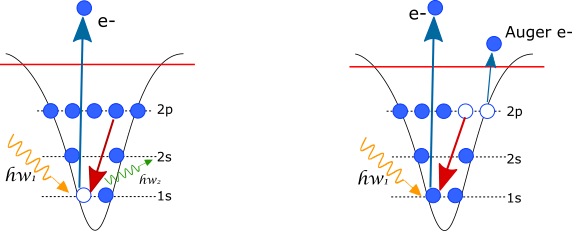
\includegraphics[width=6 cm]{../Images/text6418.png}
\caption[Relaxation processes for photoionization]{two example os the relaxation processes. On the left, A photon ionized an electron and the Electron Ein replaced, expelin a fluerecent photon in the process. on the rigth, the energie reliessed by the replacement electron is enougth to make another electron in the outer shell to also go to the continium, ASuger electron. taked form \cite{rafipoor_two-color_2017}}
\end{figure}

\subsection{Multhiphoton and tunelling Ionization}

Ionization is also possible even if one photon energy is lower than the binding potential. Electri field of lasers with intensities below $I \leqslant 10^{14}W/cm^{2}$ is not strong enougth to change the binding potzential of a atom significantly \cite{rhodes_multiphoton_1985}.  Multiphoton ionization (MPI is the simultaneous absorption of several photons to overcome the ionization barrier. The way MPI occurs in atoms depends on the laser frequency and intensity. When the intensity is much lower than the characteristic atomic resonance, MPI occurs via transitions through virtual states. Ionization by several photons at low laser intensities can be realized by the so-called resonance enhanced multiphoton ionization (REMPI)\cite{mainfray_multiphoton_nodate}.  Ionization by a REMPI process takes place in two steps
In the first step, a resonant excitation by one or more photons takes place on an electron state of the atom. In the second step, this electron state is transformed into a virtual state, to a state until the electron is excited by spontaneous decay. So for example the total energy absirbed by an electon until it gets ionizes is $n * \hbar\omega > I_{pot}$ where $n$ is the number of photon absorbes until it actially have enougth energy to overcome the potencial $I_{pot}$

For Laser intensities $I > 10^{14}W/cm^{2}$, higher intensities and lower frequencies, tunneling ionization (TI) is more likely to occur.  In this case, thebinding potential of the atom get is strongllöy afected by the electric fiels of the laser. Arround the peack of the electri field the  potential gets narrower, and the elctron in the outer states get closest to the bidding barrier. allowing the electron to tunneling througth the confining potential into de contzinium\cite{griffiths_introduction_2013}. TI is inherently a quantum process. The bending of the Coulomb potential becomes by the supperpossition of the coulomb potential and the laser field. Therefore TI must occure when the time of the ionization is shorter thatan a laser oscilation cycle\cite{berkowitz_photoabsorption_1979}. Based in the same principle, when the Laser fiel becomes so strong to lower the binding potencial that separates the highest electron level, then the electrons in this state become free electrons. This process is called barrier suppression Ionisattopn or BSI\cite{krishnan_doped_2011}.

In the fig \ref{img:ionizationprocess}, we present a scketch of the 3 possible ionization processes explained above. On the lefte we present an simple ionization process where a photon with energy $E_{phot} = \hbar\omega$ is higher than the potential barrier. In the center a MPI process is shown, $n$ photons exite the inner-shell electron, exiting it througth virtual level until it finally have enougth energy to be free to the continium. Finally on the left a TI happens. Here the coulomb potencia barrier is afectis by the laser files bending ii, The outter shell electron  gets closets to it and via tunneling  can get ionize\cite{rafipoor_two-color_2017}.

\begin{figure}[hbtp]
\label{img:ionizationprocess}
\centering
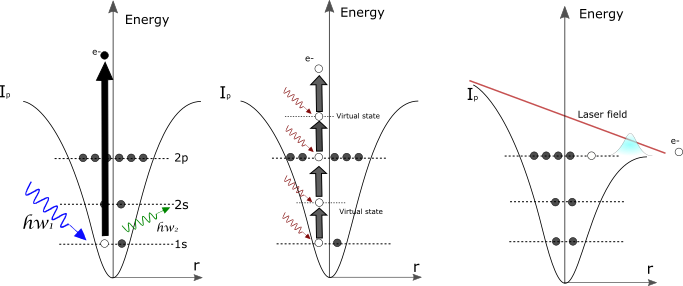
\includegraphics[width = 8 cm]{../Images/photoionization2.png}
\caption[Ionization regimes]{ On the left is the scketch of a single photon ionization process, where a photon with energy $E_{phot} = \hbar\omega$ is higher than the potential barrier $I_{p}$. On the center the MPI process,  inner-shell electron absorbs $n$ photons, getting excited througth the electronic levels (reals or virtual)  until it reach the continium. On the left the BSI Process, the coulomb potencial barrier bends by the laser fields, been lower than the outer shell electron state, the electrons can scape easilly. based on \cite{rafipoor_two-color_2017}.}
\end{figure}


As explained the Intensity of the external fiel plays an important rol in the ionizaion process. A brather eazzy whay to differenciate when each process needs to be taken into account is provides by the Keldysh parameter\cite{keldysh_ionization_1965}.

\begin{equation}
\gamma_{k}=\sqrt{\dfrac{I_{p}}{2U_{p}}}
\end{equation}

Where $\gamma_{k}$ is the Keldish parameter, $I_{p}$ is the atoms ionization potential and $U_{p}$ is the ponderomotive potential defined as

\begin{equation}
U_{p} = \dfrac{e^{2}E_{0}^{2}}{4m_{e}\omega_{0}^{2}} \propto I \lambda^{2}
\end{equation}

where $m_{e}$ is the mass of the electron, $\omega_{0}, \lambda, I$ and $E_{0}$ are the frecuency, wavelengst, intensity and the peak of the electric field of the laser pulse. On one hand, when the Keldish parameter is higher, $\gamma_{k} \gg 1$ MPI regime is conside. on the other hand, the $\gamma_{k} \ll 1$ describes the TI interaction.









\newpage
% !TeX spellcheck = en_GB
% !TeX spellcheck = en_US 


\chapter{Experimental setup}

In this chapter we will present the experimental setup used, given a special section to  the Nanodroplet generations, the doping process and the data acquisition system. A  sub-chapter is also dedicate to the single shot correlation data acquisition system tested specifically to this Master`s project.
The apparatus we worked with is part of the the  group of Molecule and Nanophysics at the University of Freiburg, Germany, and was calibrated and used for the experiments in \cite{schomas_compact_2017} and \cite{heidenreich_charging_2016}.

In figure XXX an sketch of the apparatus is shown. From left to right; The source chamber where the  ultra cold molecular beams are produced, the central chamber or "doping chamber" where the beam gas is doped via pick up process using a gas doping cell or a diffuse oven for alkaloids where gases or thermally vaporized solids and using as dopant, the last  chamber or "detection chamber" combines a VMI - TOF detection system and a  Langmuir taylor (LT) detector.
To generate the nano plasmas the apparatus was Used in two different institutions, at the Max Plank Institute for Nuclear Physics in Heidelberg and the Extreme light institute (ELI) in Szeged, Hungary, because of the special laser systems can be provided in there.

The following sections describes the essential components of the apparatus, taking special attention to the new Triggering systems implemented to correlate the VMI and TOF signals in the last part of the project.  The structure where compacted to a length of about 240 cm long, each chamber has attached its own turbo pumps with  pre-vacuum pumps and are separated by valves and skimmers. On one hand, this enables to manipulate the vacuum in an independent way and control the targets in the "detection chamber", on the other hand a allows an optimum adaptation of the suction power of the pumps to the gas load of the individual chambers as wheel as to ventilate and open, without having to disturb the entire system.

\section{Source chamber}

The Source chamber consists of a 6-way CF vacuum chamber, with a 2-stage cryostat power a cold-head that can be cooled down to 9K, located in entrance of the chamber, parallel to the floor with an attached conical nozzle for the gas expansion process. The cooling capacity of the cryostat  consists of a copper tube, into which pre-cooled helium is introduced. It can be adjusted by operating two heating resistors in combination with a sensor diode for temperature measurement and a PID controller. Controlling the resistor current the temperature at the end of the nozze can be keeping it stable. The conical nozzle used to generate the atomic beam is the standard used in the research group on Nanoplasma reasearch directed by Prf, frank Steankeirmeyer at Freiburg University.  It is made of copper and has a platinum plate on front with a hole of 5$\mu m$ of diameter for $He$ experiments and 15$\mu m$ for $Ne$ gas clusters. The diameters where choseen in order to follow the Size dependence of the \textit{Hagenas} "law",  which together with the adjustable gas pressure and the nozzle temperature regulates the flow.
The cold head-nozzle arrangement are connected to the chamber via a self-made x-y manipulator,  with a thermally insulating rubber? ring, which allows a beam adjustment in relation to the other components in the setup with out braking the vacuum. At the bottom of the chamber an "Agilent" turbo pump of $1800 L/s$ capacity is attached to a pre-vacuum scroll pump as exhaust.
A skimmer with a diameter of $400\mu m$ is located in front of the effusive jet, sorting the gas beam not just by it size but also by its velocity vectors and allowing just those beams with direction to the further vacuum chambers. To adjust the nozzle optimally to the skimmer,it is connected to an x-y displacement unit and can be aligned from outside the vacuum chamber. To prevent the small opening of the nozzle from clogging over time, high-purity helium 6.0 (99.9999$\%$ purity) and Ne 5.0 (99.999$\%$ purity)  is used and can also be used outside of the measurements ensures a constant gas flow through the nozzle. At this extreme temperatures this prevents that any impurity in the gas bottle can  condensate, blocking the nozzle or changing the conditions of the clusters production. 

\section{Dopping chamber}

As explained in the chapter above, the Doping takes place by inelastic impacts with atoms from the gas phase, referenced as the pick-up thecnique. In this experiment we doped with both metals and noble gases, and two different methods of doping are used: Metals are heated in evaporated phase in a oven, while gas dopant yield in a Gas doping cell entered the vacuum chamber through a needle valve. on the next section we will explain the elements of the dopping cham,ber and its most important characteristics used.

The oven chamber is conected after to the Source chammber via the skimmer, it is also a 6-way CF vacuum chamber, with a turbo pump  on bottom, connected to it own pre-vacum scroll pump. On the sides the flanks allows a cold trap not used in this experiment, on the other side  the flank that permit connection to the oven and the vacuum sensor. The Skimmer is made of Niquel??, a very thin metal easy to bend, so in order to prevent stronf pressures diferrence in the chamber that can modify the skimmer, a bypass is conected between the two chamber using a stainlees steel flexible hose.  
An internal stand is welded to the front of the chamber and aligned with the skimmer. This stand supports the Chopper, the gas dopping cell and the oven.
In the front the rail the choppers is located.  It is an steel  disk with three notches uniformed located,two photocell around the bottom of the disk reads the position of the bottom notches so the upper one can be positioned right in front the skimmer. In this way, when the disk rotates the beam can pass or its block by the disk  in a controlled way.  

After the chopper, there is the Gas Dopping cell, a circular flat metal base with a self modified KF hose. The base makes the base cell have a matching patter so the hose can be easy put and remove with out losing the alignment. The stainless steel flexible hose has two $5mm$ hole (one in front and one opposite to it, some cm up the base) alligned to the skimmer so the gas bean can go thought. The hose is fix to the base and goes to the top of the chamber where it is connected to a "swaglog" niddle valve that allows to control the gas flux for doping the beam. A Pfiffer CMR375 Capacitive sensor is located after the niddle valve so a better control of the pressures, ans so of the number of dopants in the cluster can be achived. This bendable construction allows not just to remove the doping cell with out difficulty but also to fit it on the top with out depending on a fix way to located the top plank, in this way there is room for maniouver and the construction is faster.

Finally at the end of the rail lies the Oven. As shown in fig XXX the oven consist on a patterned base (similar to the gas cell) that can  move a few $mm$ on $x-y$ plane. Over it, a metal cylinder with 4 heating cartridges holds a movable crucible in the center that contains the dopant sample, this movable container is set down by a rod that comes from the top of chamber after a valve. Both, the stove and crucible have holes (a conical entrance of $40mm$ diameter and $3mm$ diameter respectively) that allows the pass of the gas beam and are aligned to the beam pad, in this way  the passing Atomic beam takes dopants via collisions with vaporized sample material.

One important advantage of this new oven design done by \textit{Dominic Schomas},  is that the dopant can be change with out braking the vacuum, it was test in this experiments and prove to be useful saving time and effort. To control the temperature of the oven a temp sensor is fix in the stove, and the resistors current is manage by a PID controller allowing a stable temperature during the experiment. The maximal temperature reached was $450^{\circ}c$,  enough to creates the gas phase for the potassium K and calcium Ca used in this experiment as shown in the table XXXX. Finally there is an  extra skimmer of diameter XXX fixed to a valve between the connection of the doping chamber and the detection chamber that helps to avoid the disperse beams or an overflow from one chamber to the other.

In addition to the doped gas nano droplets, effusive gas is also released from the dopant chamber into the detector chambers through a "swarlog niidle valve" and can be ionized and detected there. This disperse gas was pour in directly on the chamber or filtered by diffusive atoms going out of the oven and passing across the second skimmer once the choppers is close. This atomic gases where added for calibration of the detectors and background reduction allowing just one gas at a time.

\section{Detection chamber}

As mentioned, the detector chamber is connected to the Oven chamber via a valve and a skimmer. The detector chamber contains a newly developed Velocity-Map-Imaging
spectrometer on top, a time-of-flight mass spectrometer on bottom and a Lt detector on front. on this section we will give a brief presentation of  the VMi and the TOf used in this experiment, but taking spacial detaile in the new Triggering process that allows us to get the single nanoplasma explotions that we are interest on. 

\subsection{Velocity map imaging VMI}

The VMI detector used in this experiment is detail in \cite{schomas_compact_2017}, this construction basically follows the standard geometry of Eppink and Parker\cite{eppink_velocity_1997}. Its composed by three electro lenses (repeler, lens and extractor) that focuses the ions or electron on a $86,6mm$ (effective area) diameter Micro channel plates (MCP) arrange. This detector set is basically  two MCPs overposed by 90 degrees each other and a phosphoscreen (PS) layer of same diameter facing the top of the chamber to a Ca-fluoride glass of $1mm$ thick, and a CCD camera focuced on the phosphorlayer. 

\begin{table}[]
\centering
\begin{tabular}{|l|l|l|l|}
\hline
\rowcolor[HTML]{EFEFEF} 
VMI & Repeler & Extractor & Lens  \\ \hline
X1  & -2430   & -1940     & 3500  \\ \hline
X3  & -7290   & 5820      & 10500 \\ \hline
Ion & 2430    & 1940      & 0     \\ \hline
\end{tabular}
\end{table}

The voltages applied to the MCP and PS determine the brightness of the final pictures of the ions, so in general just one set of voltages were use, around $1400V$ for the MCP and $4000V$ for the Ps. The achievable energy acceptance for this stack is  $34eV$ for a the VMI setting 1 and $270 eV$ for the X3 settings. The VMNI have a resolution of $\bigtriangleup E / E\leq 4\%$ \cite{schomas_compact_2017}. The camara used in the experiment was a Basler  acA1920-155um focused on the PS.

\begin{figure}[hbtp]
\label{img:mcp cut}
\centering
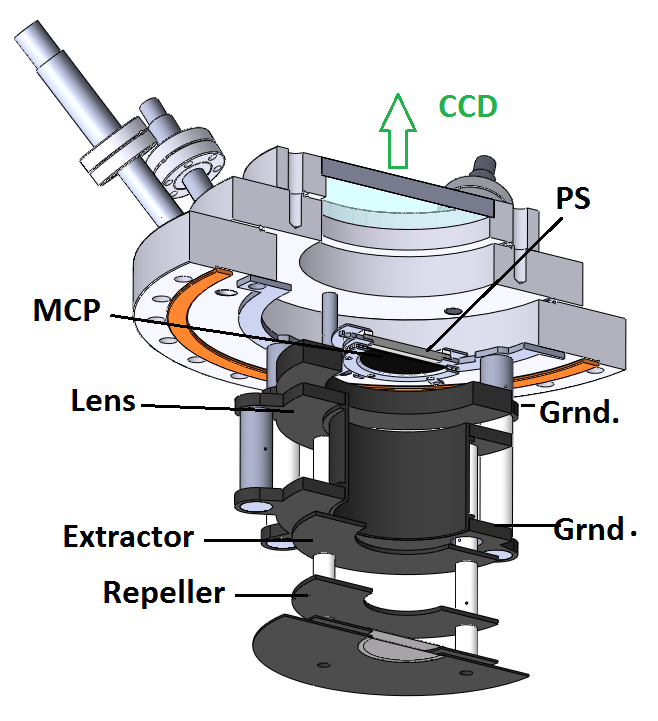
\includegraphics[scale=1]{../Images/MCP cut.png}
\caption[MCP scketckht cut]{Sectional cut view of the CAD model of the spectrometer setup. On black are the are the electrodes and the white the Polyether ether ketone (PEEK) insolators. On ornange, the cooper ring ang on blue the top window facing the cCCD camera
}
\end{figure}

On fig \ref{img:mcp cut} we present a view of the model of the VMI used in this experiment, From botom to top, the structure of the electrodes consists of two repeller electrodes separated by a few millimetres with circular openings on which a fine mesh copper grid is applied, an aperture electrode as extractor, another aperture electrode which is held at ground potential and then from the extended lens electrode with the following second ground electrode. At top  the MCP-PS arrange (o black the MCP and on gray the PS) facing the center of the window instales in the top blanck of the chamber. Around thewwindow there are three conections that allows the voltages for the electrodes and the cables are carefully arrange around tthe structure to avoid discharges or even disturb the uniform electrical field.

The openings of the repeller (on bottom in bluish color) electrodes allow the use of these electrodes as well as extractor electrodes for a TOF spectrometer. In simultaneous operation of the VMI and the TOF spectrometer, the glued grids prevent mutual field effects of the two spectrometers.  The repeller and extractor are grade 2 titanium and the lens is stainless.

\section{Time of flight spectrometer}

The TOF spectrometer used was designed by Wiley and McLaren \cite{wiley_timeflight_1955}. As it names reefers, the TOF mass spectrometer relates the time that a particle on a electric field requires to reach certain distance with its mass,  when atoms and molecules are photoionized,  they pass through an electrostatic acceleration field and are registered in a detector after crossing a field-free flight path. On the basis of the flight duration the ratio m/q of a particle can be determined as:
\begin{equation}
t-t_{0}=a\sqrt{\frac{m}{q}}
\end{equation}

Where $a$ is a experimental factor depending of the flight distance, electric fields and material of the setup,  $m/q$ is the relation mass - charge, $t_{0}$ is the time ionization time (given by the laser )and $t$ is the time of flight.

The ions creation takes place between the planar repellers and extractor aperture electrodes. Behind the extractor electrode there is a further aperture electrode, which is held at zero potential and thus generates a further flight route with a defined field, Grids are glued to the openings of the electrodes to prevent the propagation of the fields through the orifices in the electrodes. The repeller electrode is set to a positive potential and the extractor to a negative potential. The resulting electric field accelerates the ions through the openings in the flight tube, on which grids are mounted on both sides to keep the drift path free of field.
Onece the coulomb explotion takes places, the ions are accelerated by the electric field of the repeller and then fly through a field-free drift path to the detector. This allows a complete mass spectrum to be recorded within a few microseconds in a single measuring step \cite{mobius_time--flight_2016}.

\begin{figure}[hbtp]

\centering
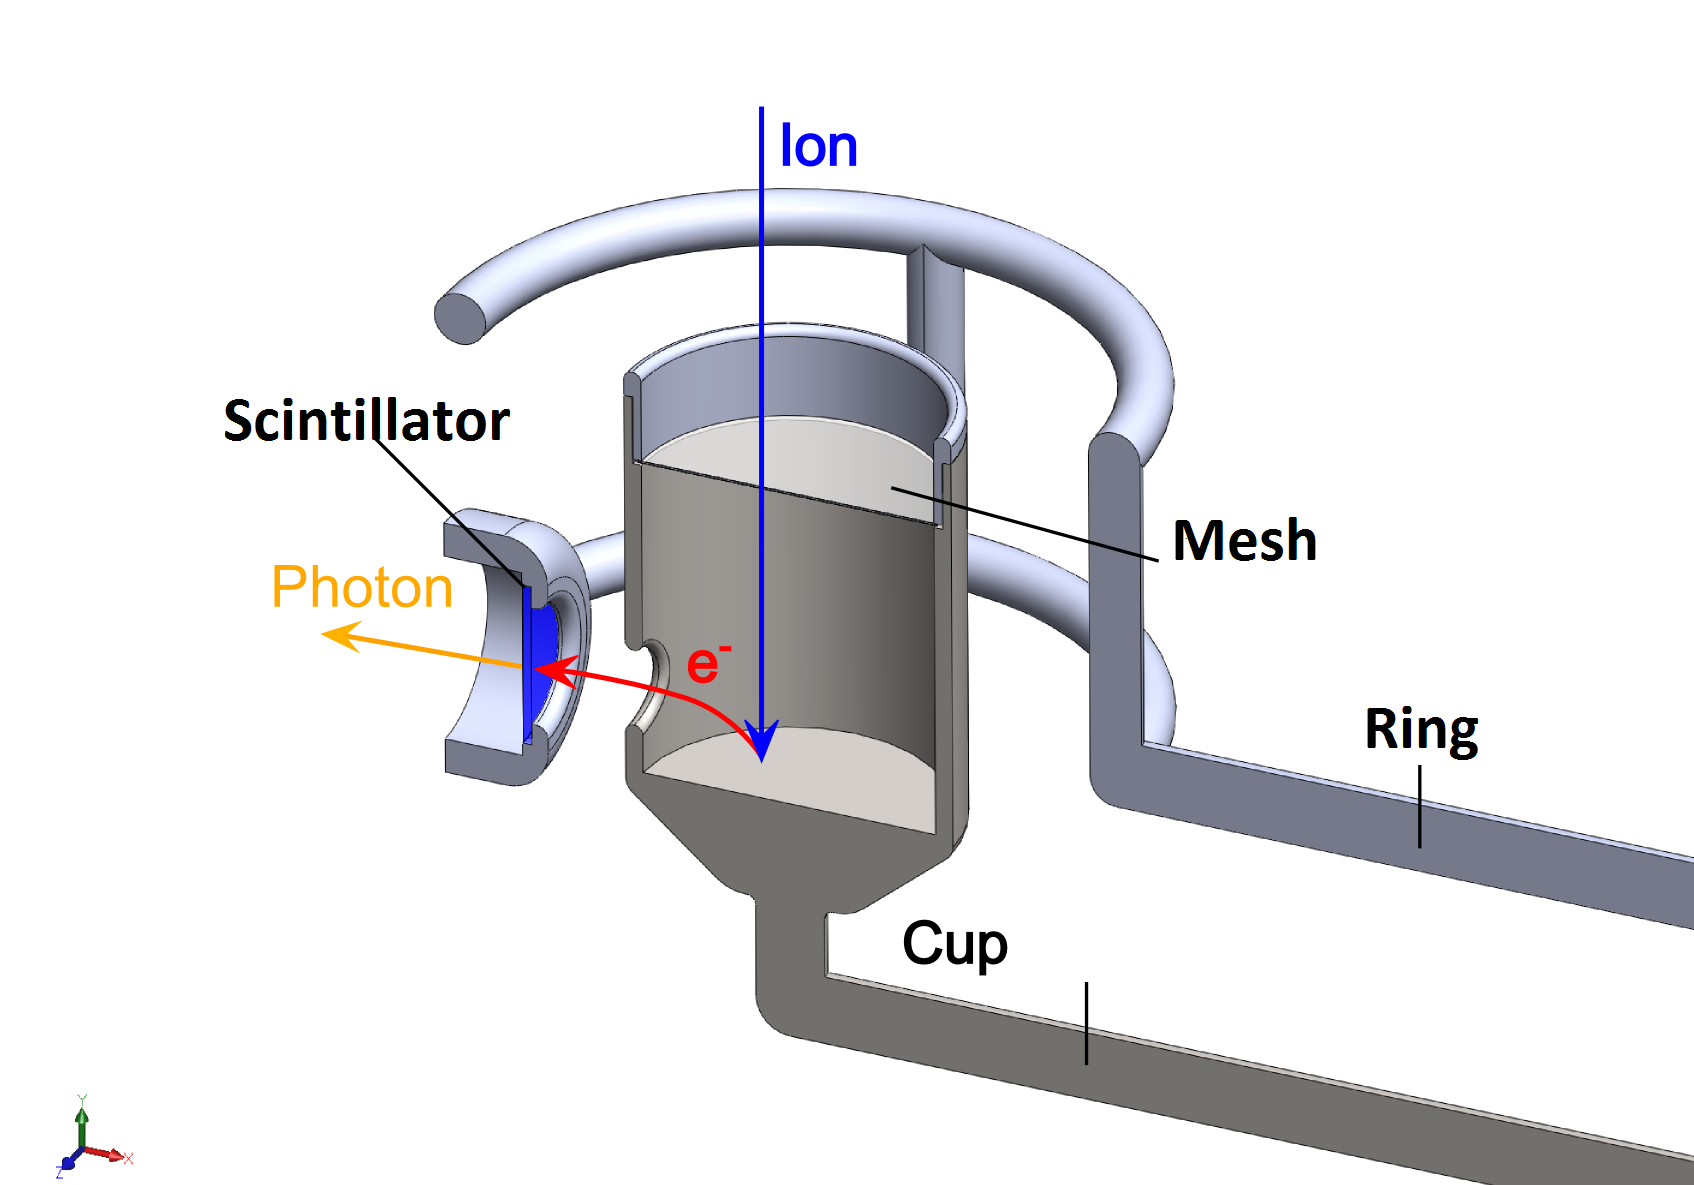
\includegraphics[scale=1]{../Images/Cup scintillator.png}
\caption[TOF cup]{Illustration of the functional principle of a Daly detector.}
\end{figure}

The flying Ions finally are detected by a  Daly detector \cite{daly_scintillation_1960}. It consists of a cup, a grid and a ring. The cup lies on negative High voltage while the ring on positive. The ions from the repeller pass trough the field free tube corrected by a drift electrosde.  Since in the direction of the hole the potential for electrons drops sharply. The ring electrode generates an E-field, which directs the ions into the cup. The ions that pass the  the grid at high speed hits on the bottom of the cup, they generate some electrons, which are transmitted through a small hole in the Cup and then in a scintillator Eljen thechnilogy(EJ-204) that flashes some photons in the process. These are detected in a Hammamatzu r-647 photomultiplier. The voltage output of the photomultiplier is controlled by a fast analog-to-digital converter, and its used at a $900V$ voltage. The cup and the drift-scintelator  tube where set at high voltages,  $-17000V$ and $-4000$ respectively.

\section{Lt detector}

The Langmuir-Taylor detector (LT detector)  chamber consists of a small CF40-6-way chamber. The detector consists essentially of an annealing filament, which is located between two planar round electrodes. The Operating Principle of an LT-Detector 
is based on surface ionisation by the tunnel effect \cite{delhuille_optimization_2002}. For the annealing filament is typically used for rhenium, platinum or tungsten, as this is the most common has a comparatively high electron work function. As a consequence, a passing neutral atoms is ionized by the heated wire, releasing an electron into the wire. The resulting ions is attracted by the negative electrodes around the wire generating a current. The ionic current generated at the electrodes is proportional to the number of ionized atoms and is measured using a picoampermeter.
The LT chamber is connected to the VMI chamber via an orifice plate and is used mainly ad a beandump also as a alingment detector. The most current generated on the chamber the most atoms arte passing thourgtthe  hole, so we can be sure that the beam pad is in the midle of the VMI repellers and extractor and the reaction takes places in the rigth area. 

\section{Camera and trigger protocol}

The idea of this master thesis was to achive individual single shots nanoplasma explosion data  in the camera (VMI) and TOF. The advantage of this correlation is the ability of threat the data in invidvidual ways, reduce the bacground in the images and achive possible properties in the coulomb explosion that are not possible when threated with averaged data.

in order to achive it, a first aproche was done doing a sofware triggering in the CCD camera software and the osciloscope for the TOF, an Acqiris Card CC103. The main idea was using LabView an external clock (a RasberryPi) was triggered by the laser, when the explosion should start, and at the same time it software trigger the camera and osciloscope programs to start the acquicition. Having all the data acquire in the same program would allow to sort the data online and reduce the storage needed to the experiment. The Labview program was tested unsusesfull for the data acquisition rate needed in ELI $100KHz$, the main problem where that using software triggering  more delay are aplied due the operating system and the comunication protocols, so even the data where acquire at the same time the delays at saving the information in the hard drive made impossible to correlate the signals.

Based on this same idea, a second aprove was used. In replacement odf a software ttrigering a ghardware triggering was used. The main idea remained, the laser triggers a dely generator that at the same time triggers the osciloscope, a R&S RTO2000 with bandwith of 600MHZ to 6GHz,  and the camara. Two facts had to been taken into account. First, our camera can´t go lower than $34\mu s$ in exposure time. Second, the timing between the camera reciving the trigger and starting the acqisition was n ot negligible as it was for thze osciloscope, as we measure, the camera took between $5-6 \mu s$ to start after the trigger was send. To solve this problem thetriggering scheme in fig XXX was used. 

\begin{table}[]
\label{tab:delaystriger}
\begin{tabular}{ll}
\multicolumn{2}{c}{List delays}                                          \\ \hline
\multicolumn{1}{|l|}{Channel} & \multicolumn{1}{l|}{Set to:}    \\ \hline
\multicolumn{1}{|l|}{A}                & \multicolumn{1}{l|}{$=T+0$}       \\ \hline
\multicolumn{1}{|l|}{B}                & \multicolumn{1}{l|}{$=T+1\mu s$}     \\ \hline
\multicolumn{1}{|l|}{C}                & \multicolumn{1}{l|}{$=B or B+6\mu s$} \\ \hline
\end{tabular}
\end{table}
A delay generator (Stanford Research Systems MD DG335) recive the laser trigger (100KHz)
channel B and C where conected to the osciloscope to chanel 1 and 2 respectivelly, and chanel A was conected to the pin 1 (trigger) on the camera. 
Lets remember that the due the minimal exposure time of the camera, we can not identify a single laser shot with it. Table \ref{tab:delaystriger} shows the deays used in the experiment, where $T$ is the original laser trigger and  A,B and C are the channels in the delay generator. In this way, it can be shown in fig, that the osciloscope can "see" each of the laser shots individually but the camera will see at least 3 shots, but fortunatelly, not each laser shot generates signal, as show in the next chapter in general just $10 to 20\%$ of the laser short ignites a plasma explosion, this mean that almos most of the pictures will have no signal, some of them can have one or more explosion, but the main of them will contain just one signal explosion in the vmi that in the data anaöisis can be correlated to its individual TOF signal. 
\begin{figure}[hbtp]
\label{fig:triggers}
\centering
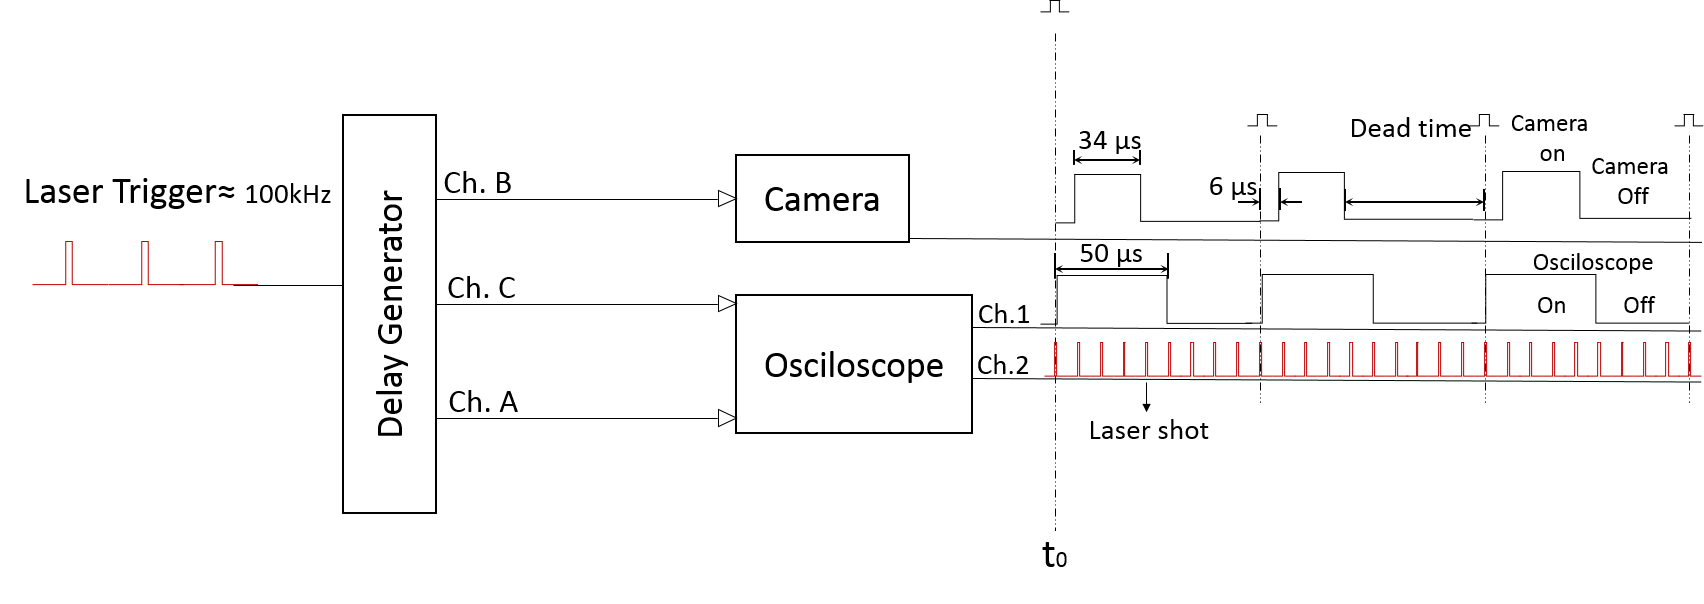
\includegraphics[scale=1]{../Images/Trigger scheme.png}
\caption[Trigger Scheme]{Schem of the trigger system used on }
\end{figure}

In Fig \ref{fig:triggers}, we show the simplies ´Trigger scheme used in the experiment. The osciloscope and camera is trigered by the delayed channel B. The osciloscope is set to $50\mu s$ and the camarta to the minimal exposure time. So the camara and osciloscope sees the same trigger, the osciloscope will record at least 5 laser shots, but the camera because starts later just can see three as shown. The pictures are saved in the memory RAM of the computer so the dead time after the camara is off is mandatory to give the operative system enougth time to save the data on disk and dont full the Ram. A small improvement in this system can be done if we trigger the camara with B and the oscilloscope with C, so both apparatus can start almost at the same time and no corrections needs to be done. Each of the data set are saved with a unique label that will help to correlate the data after. Once a explosion is found in the VMI pictures, we check in its corresponding TOF that it have just one signal in all five laser shots, so we can be sure that picture correspond to a single coulomb explosion, in case more than one signal is found, this picture is discard. 





\newpage
\include{Methods}
\newpage
\include{Messungen}
\newpage

\listoffigures
\listoftables


\bibliography{thesis}
\bibliographystyle{abbrvdin}



\chapter*{Danksagung}

An dieser Stelle Danke 
\newpage
\section*{Erklärung}

\\
\\
\\
Ort, Datum ............................... \ \ \ \ \ \ \ \ \ \ \ \ \ \ \ \ \ \ \ \ \ \ \ 
Unterschrift ................................
 
\end{document}

